\documentclass[../main.tex]{subfiles}

\begin{document}
	\section{Retroazione algebrica sullo stato}
		Dato uno sistema:
		\[
			S: 
			\begin{cases}
				\dot x &= Ax + Bu\\
				y &= Cx + Du
			\end{cases}
		\]
		\'E possibile modificare gli autovalori della matrice $ A $ dello stato, attraverso una retroazione $ u = Kx + v $ dove $ K \in \R^{n_u \times n_x} $:
		\[
			S^{*}: \footnotemark
			\begin{cases}
				\dot x &= Ax + B(Kx+v) = (A+BK)x + Bv = A^{*}x + Bv\\
				y &= Cx +D(Kx+v) = (C+DK)x + Dv = 
			\end{cases}
		\]
		\footnotetext{
			Notazione:
			\begin{itemize}
				\item $ \tilde{} $ indica le matrici relative al sistema ottenuto tramite la decomposizione di Kalman di raggiungibilit\'a.
				\item $ * $ indica le matrici relative a un sistema con la retroazione sullo stato.
			\end{itemize}}
		
		\begin{figure}[H]
			\centering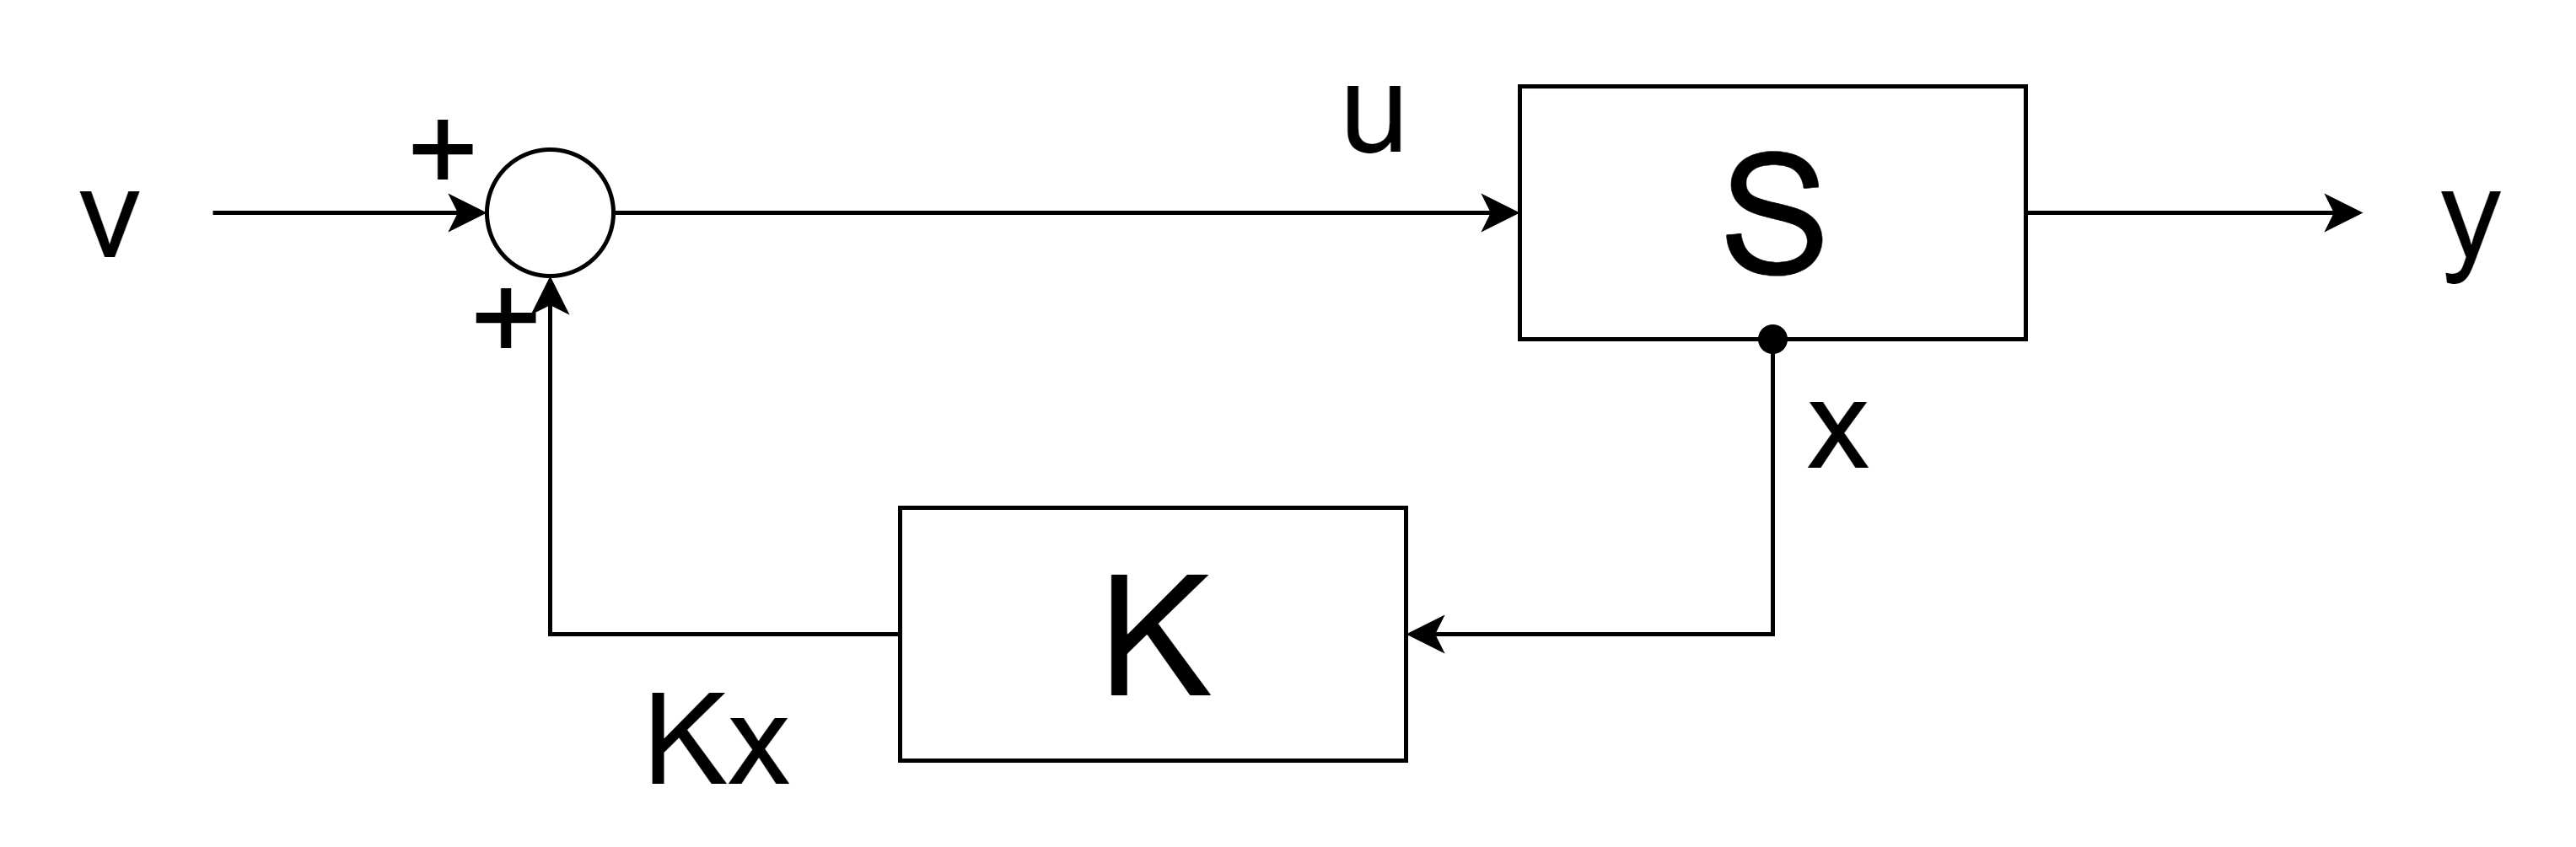
\includegraphics[width=.5\textwidth]{retroazione_algebrica_stato/retroazione_algebrica_stato}
		\end{figure}
		
		Effettuiamo la decomposizione di Kalman di raggiungibilit\'a:
		\[ x = Tz \qquad T = [T_1 | T_2] \]
		\[
			\tilde S:
			\begin{cases}
				\dot z &= \tilde Az + \tilde Bu\\
				y &= \tilde Cz + \tilde Du
			\end{cases}
		\]
		La retroazione nella nuova base diventa:
		\[ u = KTz + v = \tilde Kz + v \]
		Quindi il sistema decomposto con la retroazione sullo stato \'e:
		\[
			\tilde{S^{*}}:
			\begin{cases}
				\dot z &= (\tilde A + \tilde B \tilde K)z + \tilde Bv = \tilde{A^{*}}z + \tilde{B} v\\
				y &= \tilde{C^{*}}z + \tilde Du
			\end{cases}
		\]
		\begin{align*}
			\tilde{A^{*}} = \tilde A + \tilde B \tilde K &=
			\begin{bmatrix}
				\tilde A_{11} & \tilde A_{12}\\
				0 & \tilde A_{22}
			\end{bmatrix} +
			\begin{bmatrix}
				\tilde B_{1}\\
				0
			\end{bmatrix} K
			\begin{bmatrix}
				T_1 | T_2
			\end{bmatrix}=
			\\
			&= \begin{bmatrix}
				\tilde A_{11} & \tilde A_{12}\\
				0 & \tilde A_{22}
			\end{bmatrix} +
			\begin{bmatrix}
				\tilde B_1 K T_1 & \tilde B_1 K T_2\\
				0 & 0
			\end{bmatrix}=
			\\
			&= \begin{bmatrix}
				\tilde A_{11} + \tilde B_1 K T_1 & \tilde A_{12} + \tilde B_1 K T_2\\
				0 & \tilde A_{22}
			\end{bmatrix}
		\end{align*}
		Il polinomio caratteristico diventa:
		\begin{align*}
			\varphi^{*} &= det(sI-A^{*}) = \tilde{\varphi^{*}} = det(sI-\tilde{A^{*}}) =\\
			&= det\left[ sI - (\tilde A_{11} + \tilde B_1 K T_1) \right] \cdot \underbrace{det(sI - \tilde A_{22})}_{\varphi_{NC}}
		\end{align*}
		
	\subsection{Propriet\'a}
		\begin{itemize}
			\item
				Ho verificato che la retroazione algebrica sullo stato non modifica $ \varphi_{NC}(s) $;
			\item
				$ \varphi_C(s) $ viene modificata dalla retroazione algebrica su $ x $;
			\item 
				la retroazione algebrica sullo stato non modifica le propriet\'a di controllabilit\'a $ X_R = X_R^{*} $: ad esempio se il sistema \'e completamente controllabile, anche dopo la retroazione lo sar\'a;
			\item 
				la retroazione algebrica sullo stato pu\'o modificare le propriet\'a di osservabilit\'a (in peggio o in meglio);
			\item
				$ \varphi_C(s) $ pu\'o essere \textbf{assegnato a piacere} con una retroazione algebrica sullo stato $ x $, cio\'e \'e possibile scegliere $ K $ tale che $ det\left[ sI - (\tilde A_{11} + \tilde B_1 K T_1) \right] $ abbia autovalori arbitrari.
				
				\begin{definition}
					Definiamo \textbf{autovalori controllabili} tutti e soli gli autovalori assegnabili a piacere con retroazione algebrica sullo stato.
				\end{definition}
		\end{itemize}
	
		\begin{mdframed}[style=Esempio]
			\paragraph{Retroazione su stato che modifica l'osservabilit\'a in peggio}
			\[
				\begin{cases}
					\dot x =
					\begin{bmatrix}
						1 & 0\\
						0 & -1
					\end{bmatrix} x +
					\begin{bmatrix}
						1 & 0\\
						0 & 1
					\end{bmatrix}
					\begin{bmatrix}
						u_1\\
						u_2
					\end{bmatrix}
					\\[1em]
					y =
					\begin{bmatrix}
						1 & 1
					\end{bmatrix} x
				\end{cases}
			\]
			Studiamo l'osservabilit\'a:
			\[
				Q =
				\begin{bmatrix}
					C\\
					CA
				\end{bmatrix} =
				\begin{bmatrix}
					1 & 1\\
					1 & -1
				\end{bmatrix}
			\]
			il sistema \'e completamente osservabile perch\'e il rango di $ Q $ \'e massimo: $ rank(Q) = 2 $. Effettuiamo una retroazione sullo stato $ u = Kx + v $ con $ K = \begin{bmatrix} 0 & 0\\ 0 & 2 \end{bmatrix} $:
			\[
				(A+BK) =
				\begin{bmatrix}
					1 & 0\\
					0 & -1
				\end{bmatrix} +
				\begin{bmatrix}
					0 & 0\\
					0 & 2
				\end{bmatrix} =
				\begin{bmatrix}
					1 & 0\\
					0 & 1
				\end{bmatrix}
			\]
			Studiamo l'osservabilit\'a nel sistema retroazionato:
			\[
				Q^{*} =
				\begin{bmatrix}
					1 & 1\\
					1 & 1
				\end{bmatrix}
			\]
			$ rank(Q^{*}) = 1 $ quindi abbiamo perso osservabilit\'a.
		\end{mdframed}
		
		\begin{mdframed}[style=Esempio]
			\paragraph{Retroazione su stato che modifica l'osservabilit\'a in peggio}
			\[
				\begin{cases}
					\dot x =
					\begin{bmatrix}
						1 & 0\\
						0 & -1
					\end{bmatrix} x +
					\begin{bmatrix}
						1\\
						1
					\end{bmatrix} u
					\\[1em]
					y =
					\begin{bmatrix}
						1 & 1
					\end{bmatrix} x
				\end{cases}
			\]
			\[
				Q =
				\begin{bmatrix}
					1 & 1\\
					1 & 1
				\end{bmatrix}
				\qquad\Rightarrow\quad\text{il sistema \'e completamente osservabile}
			\]
			Effettuiamo la retroazione sullo stato $ u = kx + v $ con $ K = \begin{bmatrix} 0 & 1 \end{bmatrix} $
			\[
				A* = (A+BK) =
				\begin{bmatrix}
					1 & 0\\
					0 & -1
				\end{bmatrix} +
				\begin{bmatrix}
					1\\
					1
				\end{bmatrix}
				\begin{bmatrix}
					0 & 1
				\end{bmatrix} =
				\begin{bmatrix}
					1 & 0\\
					0 & -1
				\end{bmatrix} +
				\begin{bmatrix}
					0 & 1\\
					0 & 1
				\end{bmatrix} =
				\begin{bmatrix}
					1 & 1\\
					0 & 0
				\end{bmatrix}
			\]
			\[
				Q^{*} =
				\begin{bmatrix}
					1 & 1\\
					1 & 1
				\end{bmatrix}
				\quad\Rightarrow\quad rank(Q^{*}) = 1 
			\]
			anche in questo caso abbiamo perso osservabilit\'a.
		\end{mdframed}
		
		\begin{mdframed}[style=Esempio]
			\paragraph{Retroazione su stato che modifica l'osservabilit\'a in meglio}
			\[
				\begin{cases}
					\dot x =
					\begin{bmatrix}
						1 & 0\\
						0 & -1
					\end{bmatrix} x+
					\begin{bmatrix}
						1 & 0\\
						0 & 1
					\end{bmatrix} u
					\\[1em]
					y = 
					\begin{bmatrix}
						1 & 0
					\end{bmatrix} x
				\end{cases}
			\]
			Studiamo l'osservabilit\'a:
			\[
				Q = 
				\begin{bmatrix}
					1 & 0\\
					1 & 0
				\end{bmatrix}
			\]
			il sistema non \'e completamente osservabile. Applichiamo quindi una retroazione algebrica sullo stato: $ u = Kx + v $
			\[
				A^{*} = A+BK = A+IK = A + K
			\]
			Potendo scegliere a piacere gli elementi di $ K $, sommiamo ad $ A $, una costante arbitraria. Per esempio: $ K \triangleq \begin{bmatrix} 0 & 1\\ 0 & 0 \end{bmatrix} $
			\[
				A^{*} = 
				\begin{bmatrix}
					1 & 1\\
					0 & -1
				\end{bmatrix}
				\quad\Rightarrow\quad
				Q^{*} =
				\begin{bmatrix}
					1 & 0\\
					1 & 1
				\end{bmatrix}
			\]
			Il rango di $ Q^{*} $ \'e massimo quindi il sistema retroazionato \'e completamente osservabile.
		\end{mdframed}
	
		\begin{mdframed}[style=Esempio]
			\paragraph{Retroazione su stato che modifica l'osservabilit\'a in meglio}
			\[
				\begin{cases}
					\dot x =
					\begin{bmatrix}
						0 & 0\\
						0 & 0
					\end{bmatrix} x+
					\begin{bmatrix}
						1\\
						0
					\end{bmatrix} u
					\\[1em]
					y = 
					\begin{bmatrix}
						1 & 0
					\end{bmatrix} x
				\end{cases}
			\]
			\[
				Q=
				\begin{bmatrix}
					1 & 0\\
					0 & 0
				\end{bmatrix}
			\]
			Il sistema non \'e completamente osservabile. Applichiamo la retroazione sullo stato e scegliamo: $ K \triangleq \begin{bmatrix} 0 & 1 \end{bmatrix} $, cio\'e $ u = x_2 + v $. Prima $ x_1 $ dipendeva solo da $ u $, ma non da $ x_2 $, mentre adesso $ x_2 $ dipende da $ x_1 $, perch\'e $ u $ dipende da $ x_1 $.
			\[
				A^{*} = A+BK = 
				\begin{bmatrix}
					0 & 0\\
					0 & 0
				\end{bmatrix} + 
				\begin{bmatrix}
					1\\
					0
				\end{bmatrix}
				\begin{bmatrix}
					0 & 1
				\end{bmatrix} = 
				\begin{bmatrix}
					0 & 1\\
					0 & 0
				\end{bmatrix}
				\quad\Rightarrow\quad
				Q^{*} =
				\begin{bmatrix}
					C\\
					CA^{*}
				\end{bmatrix} =
				\begin{bmatrix}
					1 & 0\\
					0 & 1
				\end{bmatrix}
			\]
			il rango di $ Q^{*} $ \'e 2, allora il sistema \'e completamente osservabile.
		\end{mdframed}
		
	\subsection{Sistema stabilizzabile}
		Un sistema \'e \textbf{stabilizzabile} (cio\'e \'e possibile renderlo asintoticamente stabile) se e solo se la sua parte non controllabile \'e asintoticamente stabile ($ \Leftrightarrow $ gli autovalori di $ \varphi_{NC}(s) $ sono tutti a $ \Re < 0 $).
	
	\subsection{Esercizi}
		\begin{document}
	\begin{mdframed}[style=Exercise]
		\begin{Exercise}[title={Studio completo del sistema e stabilizzazione}, difficulty=3]
			\[
				\begin{cases}			
					\dot x &=
					\begin{bmatrix}
						0 & 0 & 1\\
						0 & -1 & 0\\
						0 & 1 & 0
					\end{bmatrix} x+
					\begin{bmatrix}
						0 & 1\\
						0 & 0\\
						1 & 0
					\end{bmatrix} u
					\\[.75cm]
					y &=
					\begin{bmatrix}
						0 & 1 & 0\\
						1 & 1 & 0
					\end{bmatrix} x
				\end{cases}
				\qquad\qquad
				\begin{aligned}
					n_x &= 3\\
					n_u &= 2\\
					n_y &= 2
				\end{aligned}
			\]
			
			\paragraph{Stabilit\'a}
				Per calcolare gli autovalori del sistema possiamo procedere in due modi:
				\begin{enumerate}
					\item
						notiamo che $ A $ \'e una matrice triangolare a blocchi: $ [0]\ \text{e}\ \begin{bmatrix} -1 & 0\\ 1 & 0 \end{bmatrix} $, dove il secondo blocco \'e a sua volta triangolare. Quindi gli autovalori sono gli elementi della diagonale: $ 0, -1, 0 $.
					\item
						\[
							\varphi(s) = det(sI-A) = det
							\begin{bmatrix}
								s & 0 & -1\\
								0 & s+1 & 0\\
								0 & -1 & s
							\end{bmatrix} = s^2(s+1)
						\]
						\[ 
							\text{Gli autovalori sono:}
							\begin{cases}
								s_{1,2} = 0\\
								s_2 = -1
							\end{cases}
						\]
				\end{enumerate}
				
				Poich\'e un autovalore ha $ \Re = 0 $, il sistema non sar\'a asintoticamente stabile. Per determinare il tipo di stabilit\'a dobbiamo studiare il polinomio minimo $ m(s) $. Si possono seguire pi\'u strade:
				\begin{itemize}
					\item
						Sappiamo che $ m(s) \subseteq\cdot \varphi(s) $, quindi i possibili polinomi minimi sono: $ s^2(s+1) $ e $ s(s+1) $.\\ Inoltre $ m(s) $ deve essere polinomio annullante per $ A $, quindi possiamo trovare quale dei due \'e quello corretto verificando questa propriet\'a: se $ A(A+1) = 0 $, allora $ m(s) = s(s+1) $, se invece $ A^2(A+I) = 0 $, allora $ m(s) = s^2(s+1) $.
					\item
						calcolandolo attraverso $ (sI-A)^{-1} $:
						\[
							(sI-A)^{-1}=
							\begin{bmatrix}
								\dfrac{1}{s} & \dfrac{1}{s^2(s+1)} & \dfrac{s+1}{s^2(s+1)}\\[.5cm]
								0 & \dfrac{1}{s+1} & 0\\[.5cm]
								0 & \dfrac{s}{s^2(s+1)} & \dfrac{1}{s}
							\end{bmatrix} =
							\begin{bmatrix}
								\dfrac{1}{s} & \dfrac{1}{s^2(s+1)} & \dfrac{1}{s^2}\\[.5cm]
								0 & \dfrac{1}{s+1} & 0\\[.5cm]
								0 & \dfrac{1}{s(s+1)} & \dfrac{1}{s}
							\end{bmatrix}
						\]
						\[ \Rightarrow\quad m(s) = mcm\left\lbrace s, s^2, s(s+1), s^2(s+1), (s+1) \right\rbrace  = s^2(s+1) \]
				\end{itemize}
				Poich\'e $ m(s) $ ha una radice a $ \Re = 0 $ con molteplicit\'a 2, il sistema \'e instabile.
				
			\paragraph{Raggiungibilit\'a/Controllabilit\'a}
				\[
					(sI-A)^{-1}B =
					\begin{bmatrix}
						\dfrac{1}{s} & \dfrac{1}{s^2(s+1)} & \dfrac{1}{s^2}
						\\[1em]
						0 & \dfrac{1}{s+1} & 0
						\\[1em]
						0 & \dfrac{1}{s(s+1)} & \dfrac{1}{s}
					\end{bmatrix}
					\begin{bmatrix}
						0 & 1
						\\[1em]
						0 & 0
						\\[1em]
						1 & 0
					\end{bmatrix} =
					\begin{bmatrix}
						\dfrac{1}{s^2} & \dfrac{1}{s}
						\\[1em]
						0 & 0
						\\[1em]
						\dfrac{1}{s} & 0
					\end{bmatrix}
				\]
				\[
					\varphi_C(s) = s^2 \qquad \varphi_{NC}(s) = s+1
				\]
				Quindi $ s_{1,2} = 0 $ sono gli autovalori controllabili, mentre $ s_3 = -1 $ \'e l'unico autovalore non controllabile. Si poteva gi\'a intuire dalla seconda equazione del sistema $ \dot x = -x_2 $, a cui era associato l'autovalore $ s_3 $. Infatti la componente $ x_2 $ dello stato \'e indipendente dalle altre componenti e non dipende dal controllo.
				
				\[
					n_R = \pDeg{\varphi_C(s)} = 2 \equiv n_u \quad\Rightarrow\quad X_R = B =
					\begin{bmatrix}
						0 & 1\\
						0 & 0\\
						1 & 0
					\end{bmatrix}
				\]
				
			\paragraph{Stabilizzazione}
				La parte non controllabile \'e gi\'a stabile, quindi con una retroazione sullo stato $ u = Kx + v $ \'e possibile rendere il sistema asintoticamente stabile.
				\[ S^{*}: \dot x = (A+BK)x + Bv = A^{*}x + B^{*}u \]
				\[ x: 3 \times 1 \quad u: 2 \times 1 \quad\Rightarrow\quad K: 2 \times 3 \]
				\[
					\begin{aligned}
						A^{*} = (A+BK) &=
						\begin{bmatrix}
							0 & 0 & 1\\
							0 & -1 & 0\\
							0 & 1 & 0
						\end{bmatrix} +
						\begin{bmatrix}
							0 & 1\\
							0 & 0\\
							1 & 0
						\end{bmatrix}
						\begin{bmatrix}
							k_{11} & k_{12} & k_{13}\\
							k_{21} & k_{22} & k_{23}
						\end{bmatrix} =
						\\
						&= \begin{bmatrix}
							k_{21} & k_{22} & k_{23}\\
							0 & 0 & 0\\
							k_{11} & k_{12} & k_{13}
						\end{bmatrix} =
						\begin{bmatrix}
							k_{21} & k_{22} & 1 + k_{23}\\
							0 & -1 & 0\\
							k_{11} & 1 + k_{12} & k_{13}
						\end{bmatrix}
						\\
						B^{*} &\equiv B =
						\begin{bmatrix}
							0 & 1\\
							0 & 0\\
							1 & 0
						\end{bmatrix}
					\end{aligned}
				\]
				
				\'E evidente che il sistema non \'e completamente controllabile, perch\'e la seconda componente dello stato non dipende dal controllo e dalle altre componenti dello stato: $ \dot{x_2} = x_2 $. Infatti le propriet\'a di controllabilit\'a non cambiano con retroazioni algebriche sullo stato.
				
				Calcoliamo il nuovo polinomio caratteristico:
				\begin{align*}
					\varphi^{*}(s) &= det(sI-A^{*}) =\\
					&= det
					\begin{bmatrix}
						s-K_{21} & -K_{22} & -(1+K_{23})\\
						0 & s+1 & 0\\
						-K_{11} & -(1+K_{12}) & s-K_{13}
					\end{bmatrix} =\\
					&= (s+1)\left[ (s-K_{21})(s-K_{13}) - K_{11}(1+K_{23}) \right] =\\ 
					&= (s+1)\left[ s^2 - (K_{21}+K_{13})s + K_{21}K_{13} - K_{11}(1+K_{23}) \right]
				\end{align*}
				La retroazione assegna tutti e soli gli autovalori controllabili: infatti $ (s+1) $, la parte non controllabile \'e rimasta tale. Posso imporre che il polinomio sia equivalente a qualunque polinomio monico di secondo grado:
				\[ s^2 - (K_{21}+K_{13})s + K_{21}K_{13} - K_{11}(1+K_{23}) = s^2 + bs + c \qquad \text{con}\ b,c \in \R \]
				\[
					\begin{cases}
						-(K_{21} + K_{13}) = b\\
						K_{21} K_{13} - K_{11}(1+K_{23}) = c
					\end{cases}
				\]
				Prima scegliamo $ K_{21} $ e $ K_{13} $ in modo che sia verificata la prima equazione. Quindi possiamo scegliere $ K_{11} $ e $ K_{23} $ in modo che anche la seconda equazione sia verificata: $ K_{11}(1+K_{23}) = c - K_{21}K_{13} $.
		\end{Exercise}
	\end{mdframed}
\end{document}
\end{document}